\section{Business architecture}
\label{sec:business-architecture}

	\subsection{Prototypical business structure}
	
	Following the metaphor of layers presented in the motivation view, we decided to explain the  organisation of business structure in terms of layers as well. Figure \ref{fig:business-structure-protopypical} depicts three layers with the most important elements of the business structure. 
	
	\begin{figure}[h]
		\centering
		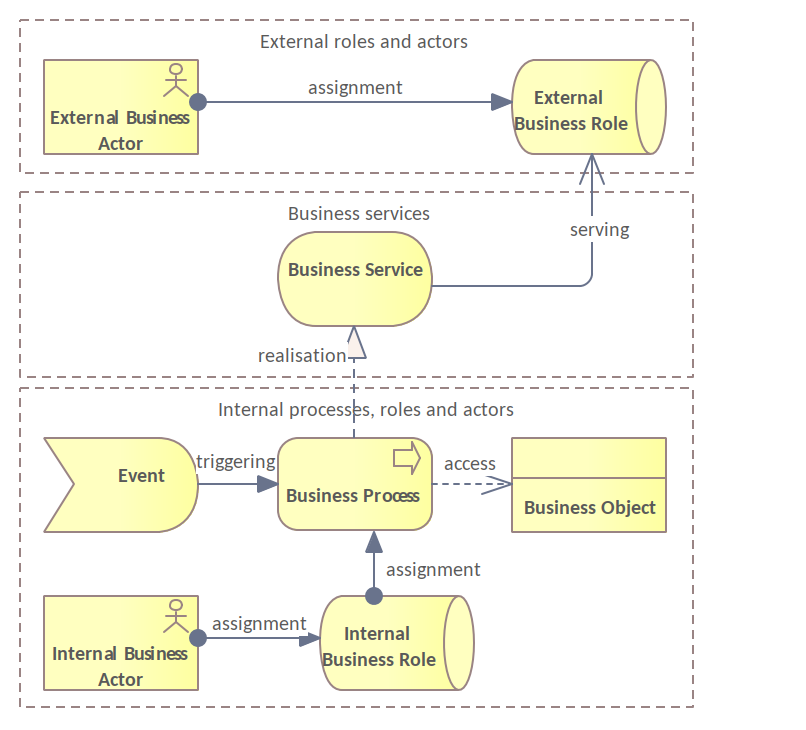
\includegraphics[width=0.67\textwidth]{images/views/Business view.png}
		\caption{The prototypical business structure view}
		\label{fig:business-structure-protopypical}
	\end{figure} 
	
	The topmost layer accounts for the external players or \textit{actors}, which represent a business entity that is capable of performing behaviour, and \textit{roles}, which represent skills and responsibilities for performing specific behaviour, and to which an actor can be assigned \citep{archimate3.1}. 
	
	The middle layer represents the \textit{services} that are offered by the organisation to the external players. A business service represents explicitly defined behaviour that a business role, business actor, or business collaboration exposes to its environment \citep{archimate3.1}.
	
	The lower layers accounts for the internal organisation in terms of \textit{events}, \textit{roles}, \textit{processes} and \textit{objects}. The business process represents a sequence of business behaviours that achieves a specific result such as a defined set of products or business services. The business event represents an organizational state change; while a business object represents a (passive) concept used within a particular business domain.
	
	In the current section we focus almost entirely on the bottom layer describing internal processes, events and roles answering the questions who shall do what and when. 
	
	Moreover, from here onwards, we start laying out two perspectives. First a baseline representing the current setup and, second, how the new processes will look like in the light of digital transformations moving towards goals identified in the motivation structure (Section \ref{sec:motivation-architecture}).
	
	\subsection{Current asset lifecycle stages}
	\label{sec:lifecycle-current-stages}
	
	\begin{figure}[h]
		\centering
		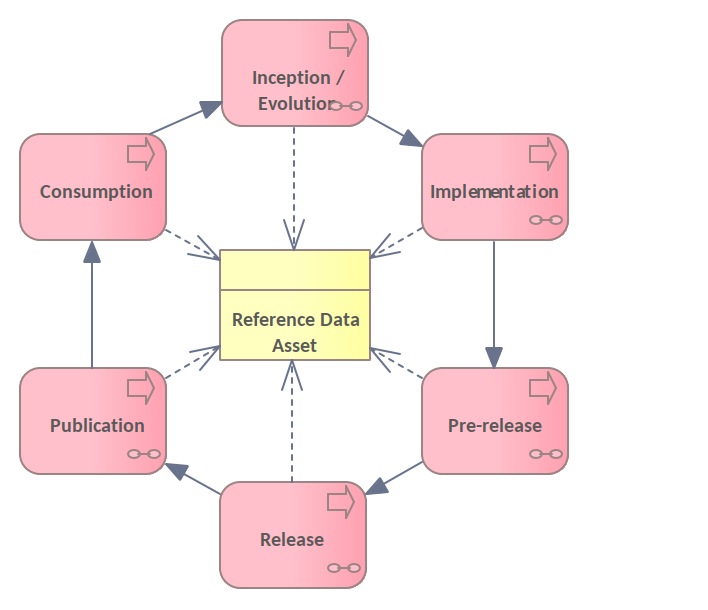
\includegraphics[width=0.67\textwidth]{images/business/Lifecycle process only (current).png}
		\caption{The current asset lifecycle stages}
		\label{fig:lifecycle-current-stages}
	\end{figure} 

	\subsection{Actors and roles}
	\label{sec:lifecycle-roles}	
	
	\begin{figure}[h]
		\centering
		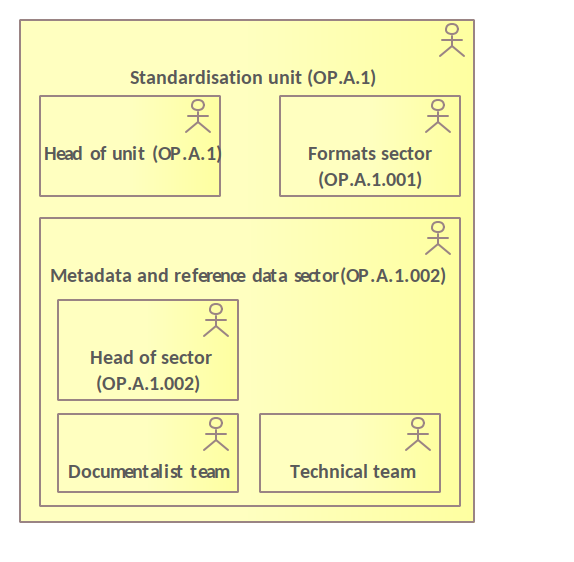
\includegraphics[width=0.47\textwidth]{images/business/Internal Business Actors.png}
		\caption{The actors in metadata and reference data sector}
		\label{fig:actors-team}
	\end{figure} 

	\begin{figure}[h]
		\centering
		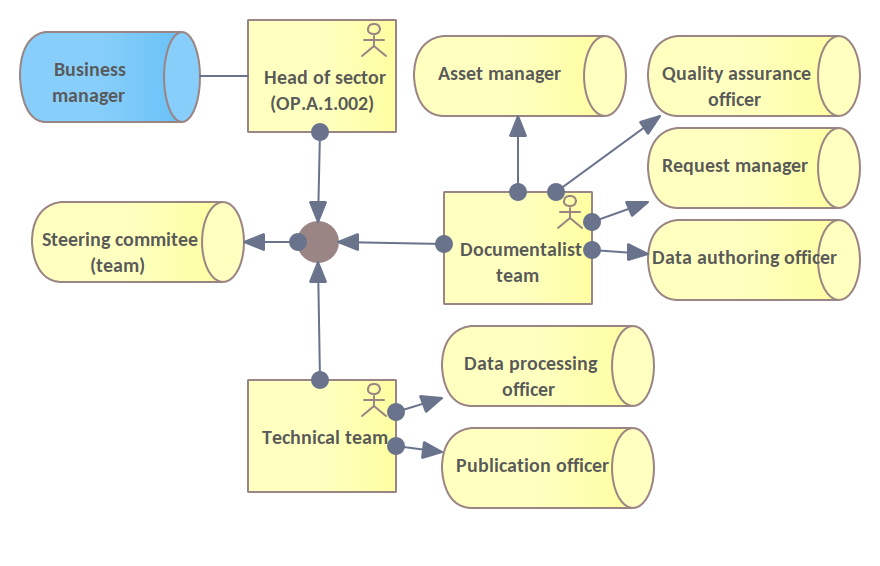
\includegraphics[width=0.7\textwidth]{images/business/Internal Roles.png}
		\caption{The internal roles in metadata and reference data sector}
		\label{fig:internal-roles}
	\end{figure}

	\begin{figure}[h]
		\centering
		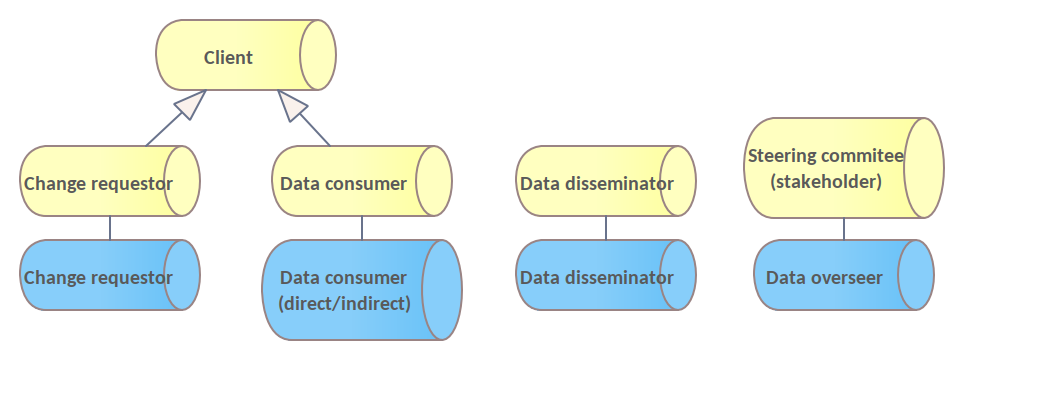
\includegraphics[width=0.7\textwidth]{images/business/External Roles.png}
		\caption{The external roles to standardisation unit}
		\label{fig:external-roles}
	\end{figure} 
	
	\subsection{Current asset lifecycle}
	\label{sec:lifecycle-current}

	\begin{figure}[h]
		\centering
		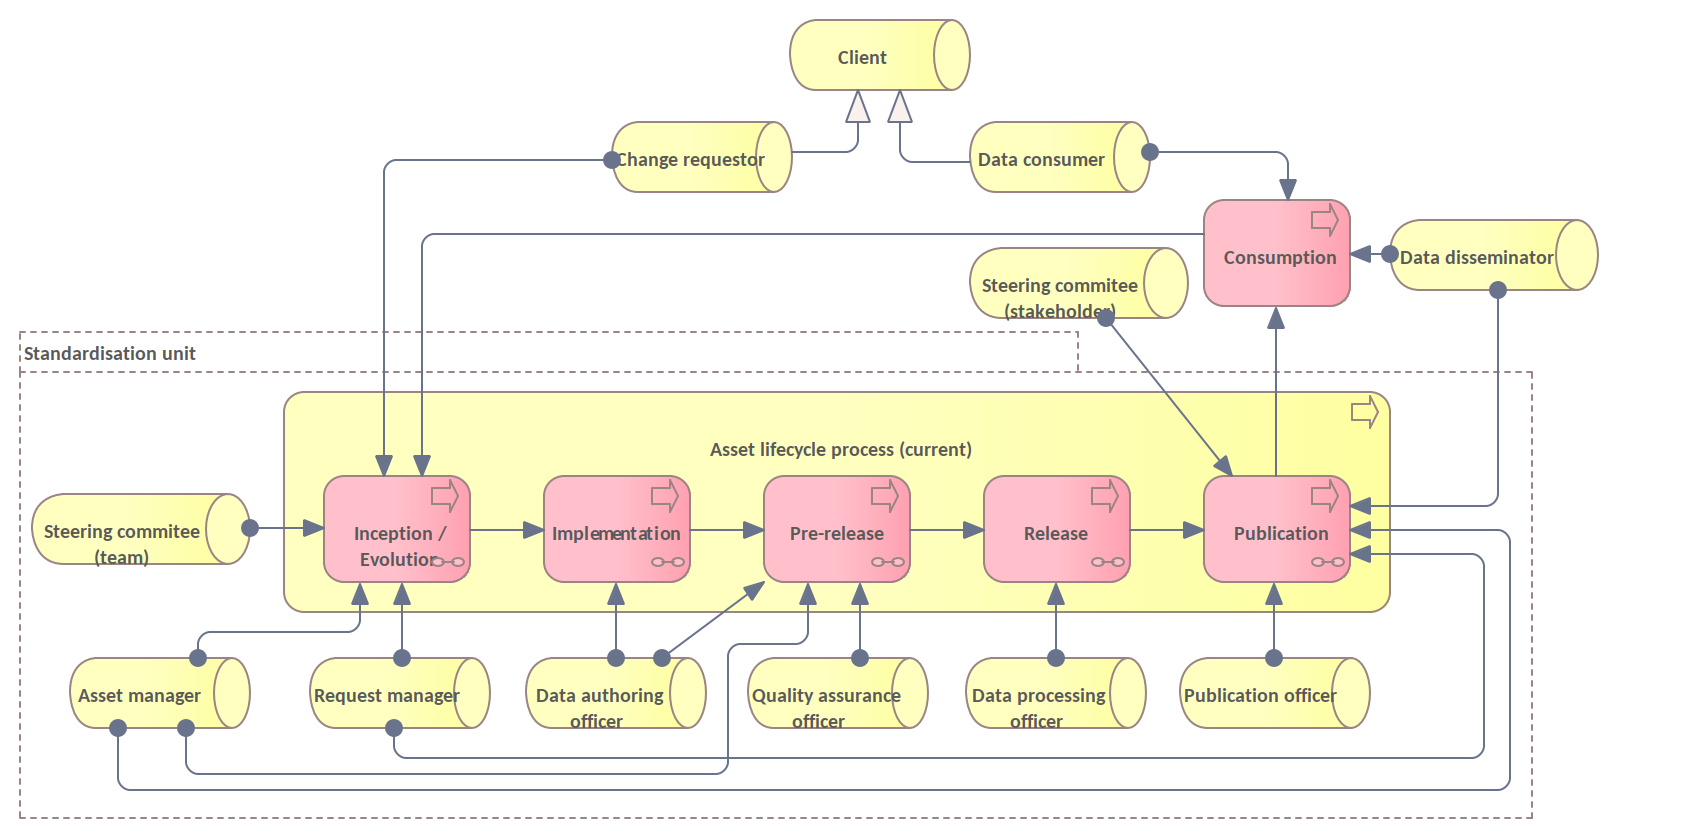
\includegraphics[width=1.05\textwidth]{images/business/Lifecycle (current).png}
		\caption{The current asset lifecycle stages and roles}
		\label{fig:lifecycle-current}
	\end{figure} 
	